\chapter{Resonance in RLC Circuits}
\begin{figure}
  \centering
  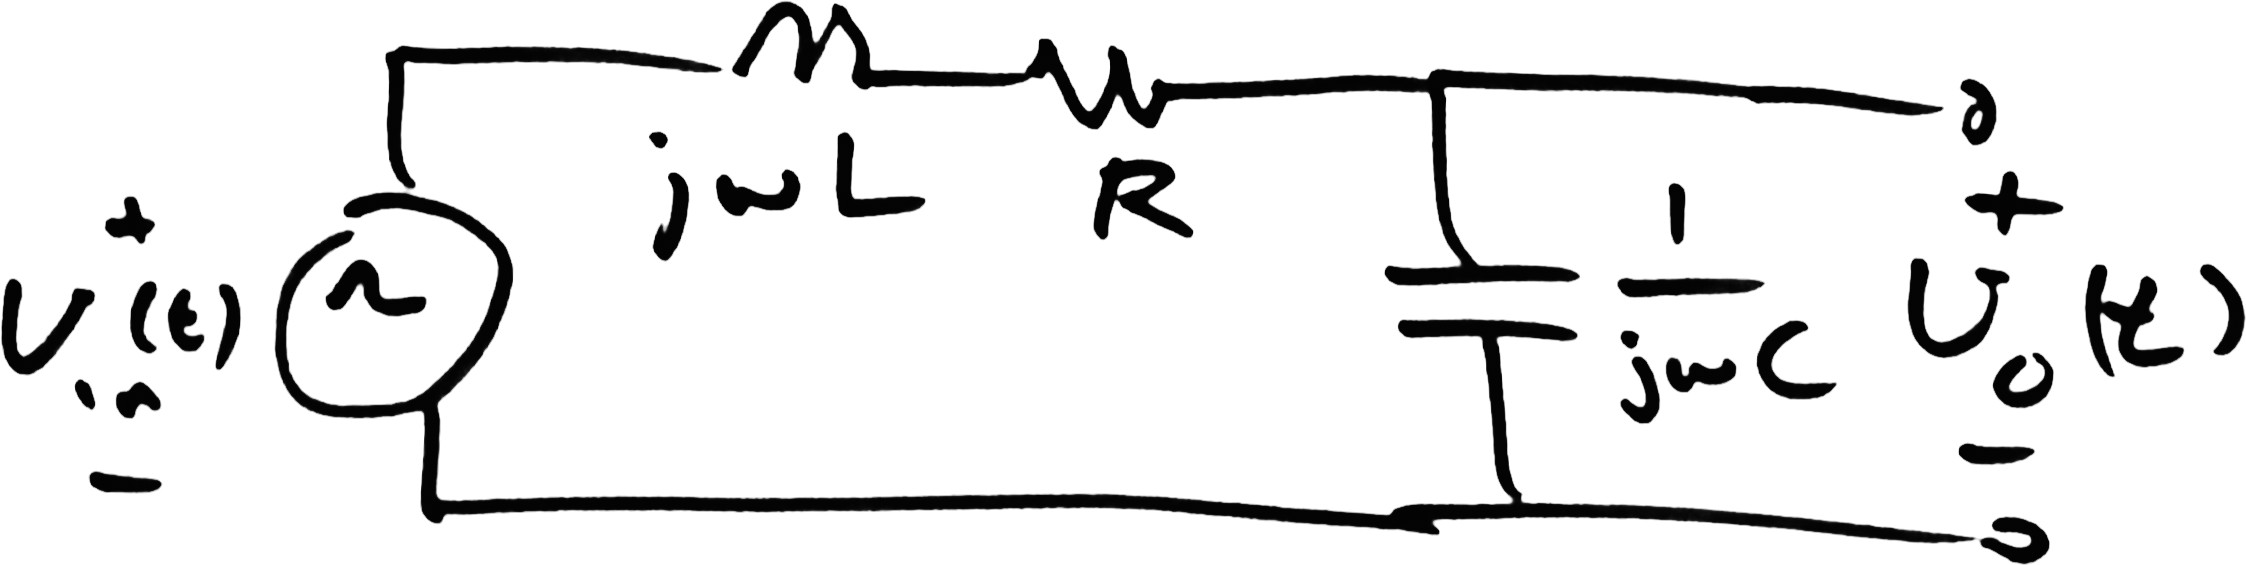
\includegraphics[width=0.7\linewidth]{figures/10/lrc}
  \caption{An LRC circuit.}
  \label{figure:lec10-lrc}
\end{figure}

To analyze the LRC circuit in
\autoref{figure:lec10-lrc}, assign phasors to both
\(v_\text{in}\) and
\(v_\text{o}\):
\begin{align}
  v_\text{in}(t) &= \Re\sbr{\underbrace{V_\text{in}}_{\text{phasor}} e^{j\omega t}} \\
  v_\text{o}(t) &= \Re\sbr{\underbrace{V_\text{o}}_{\text{also phasor}} e^{j\omega t}}
  \intertext{\(V_\text{o}\) spans the rightmost leg of a a three-way voltage  divider (\(V_\text{in}\) among impedances \(j\omega L\), \(R\), and \(\frac{1}{j\omega C}\), so the transfer function is the following impedance ratio:}
  \frac{V_\text{o}}{V_\text{in}}
  = H(j\omega)
  &= \frac{\frac{1}{j\omega C}}{\frac{1}{j\omega C} + R + j\omega L} \\
  &= \frac{1}{LC\del{j\omega}^2 + j\omega RC + 1}
\end{align}

\section{Time-domain analysis}
\subsection{Eigenvalues, two ways}
\begin{figure}
  \centering
  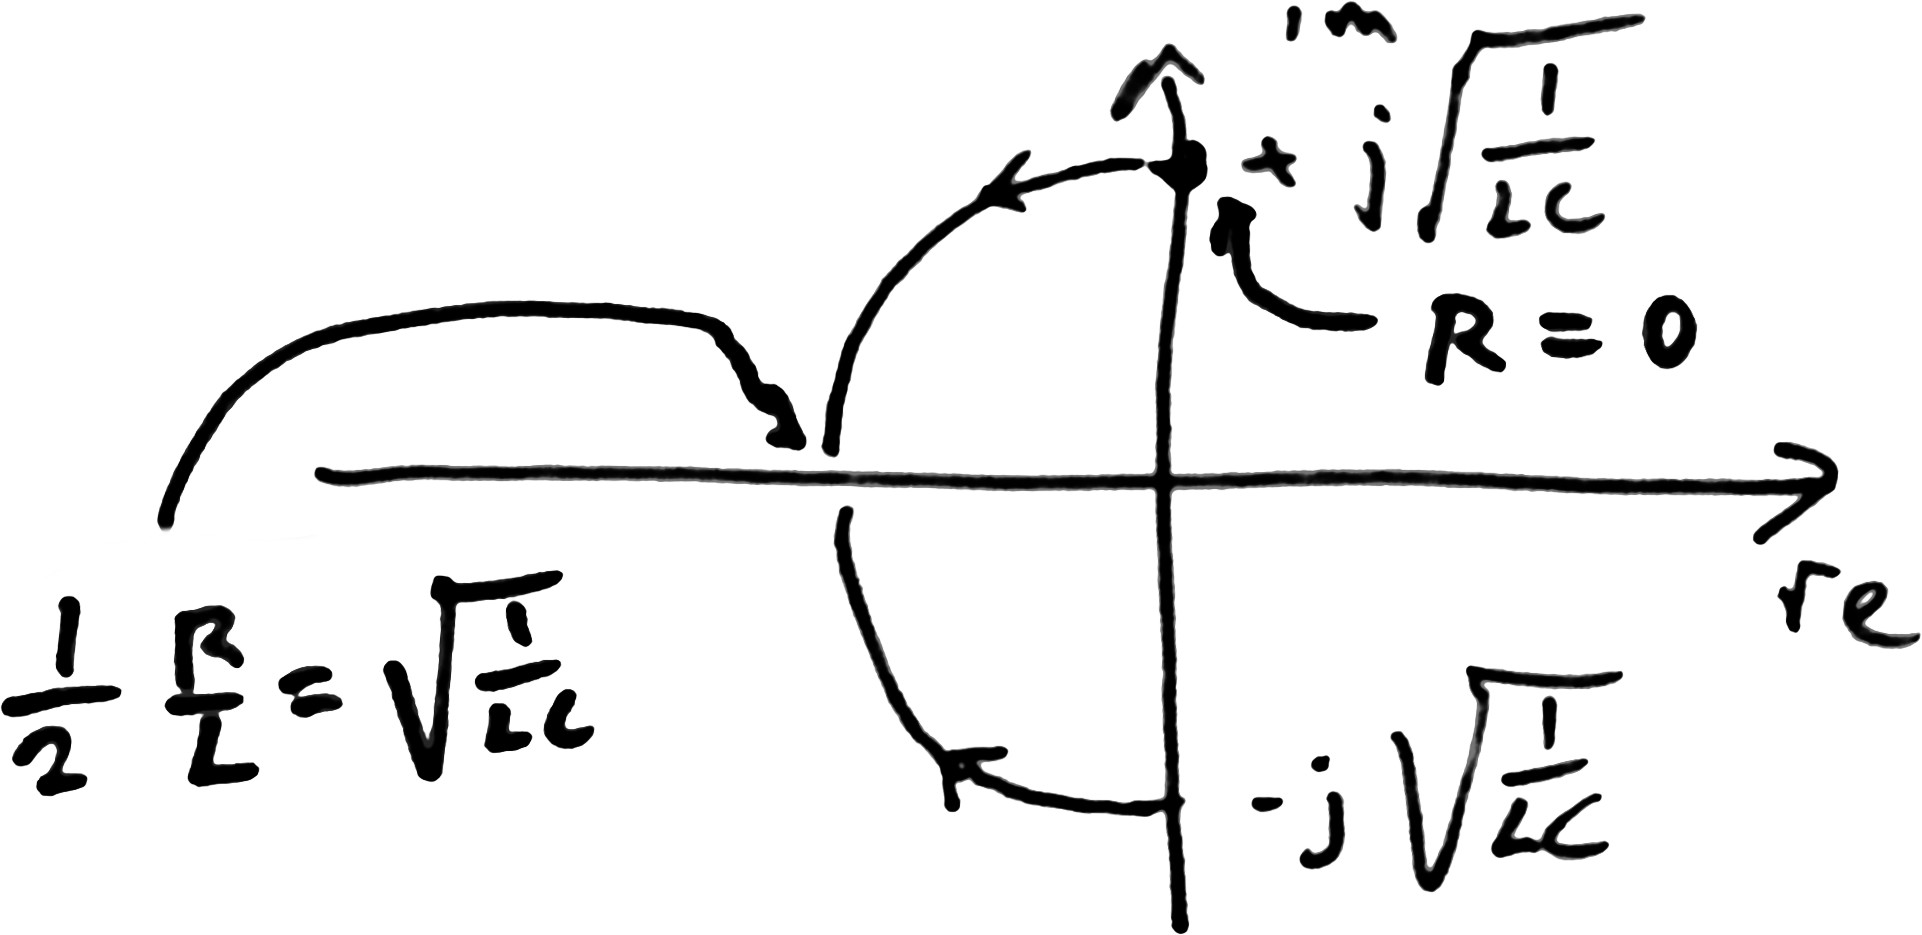
\includegraphics[width=0.6\linewidth]{figures/10/root-locus}
  \caption{Eigenvalue locus from imaginary pair at \(R =0\) to negative real at critical \(R\), as \(R\) increases from \(0\).}
  \label{figure:lec10-lrc}
\end{figure}
In \autoref{eq:lec7-lrc-A}, we found a state space differential equation model of this circuit with the following matrix:
\begin{align}
  A
&= \begin{bmatrix}
    \phantom{-}0 & \phantom{-}\frac{1}{C} \\[3pt]
    -\frac{1}{L} & -\frac{R}{L}
  \end{bmatrix} \\
  \intertext{Its eigenvalues,}
  \lambda_{1,2}
  &= -\frac{1}{2} \frac{R}{L} \pm j\sqrt{\del{\frac{1}{2}\frac{R}{L}}^2 - \frac{1}{LC}}
  \intertext{are a complex conjugate pair on the imaginary axis when \(R = 0\). As \(R\) approches a critical value, they slowly approach the same point on the negative real axis. Their rendezvous is depicted in
  \autoref{figure:lec10-lrc}. (Afterwards, they separate but remain real and negative.)
  We will reparameterize these eigenvalues in a way that traces their trajectory.
  Call the undamped (angular) frequency \(\omega_n\):}
  \eval{\lambda_{1,2}}_{R = 0}
  &= \pm \sqrt{-\frac{1}{LC}} = \pm j \omega_n,
  \intertext{and define a damping coefficient \(\xi\) (\href{https://en.wikipedia.org/wiki/Xi\_(letter)}{Greek letter xi}) that goes from 0 to 1 as the two eigenvalues leave the imaginary axis and meet at a negative real.}
  \xi &= \frac{1}{2} \frac{R}{\sqrt{\frac{L}{C}}}
\end{align}
This parameterization appears in \autoref{figure:lec10-root-locus-reparam}.

\begin{figure}
  \centering
  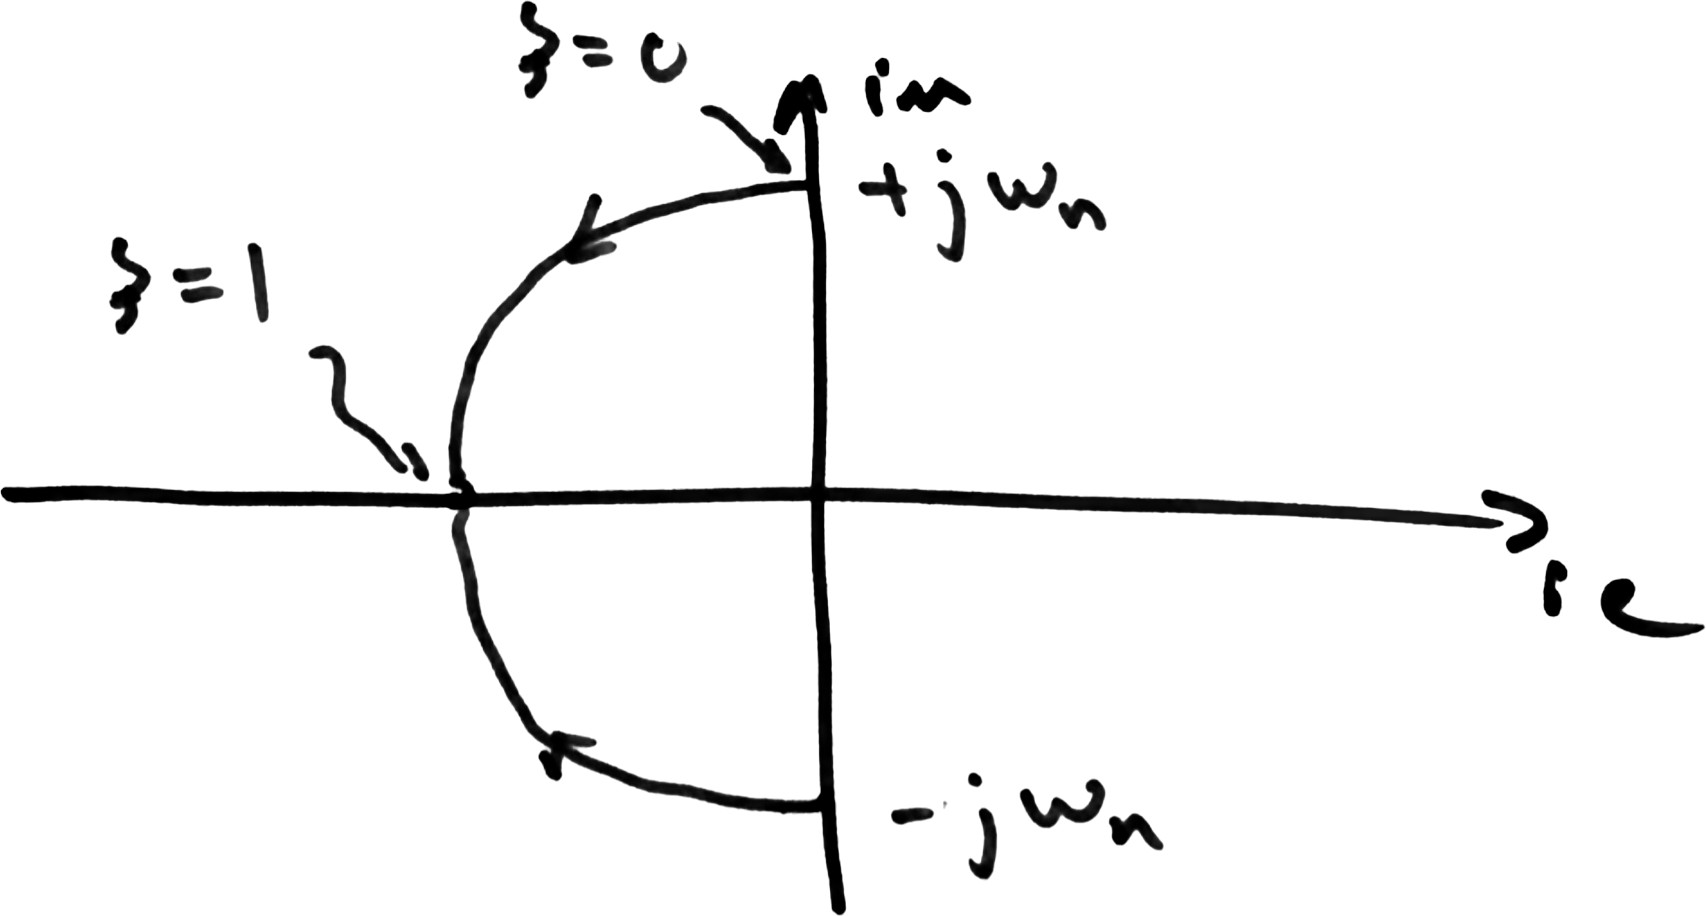
\includegraphics[width=0.6\linewidth]{figures/10/root-locus-reparam}
  \caption{\autoref{figure:lec10-lrc}, but reparameterized using \(\omega_n\) and \(\xi\).}
  \label{figure:lec10-root-locus-reparam}
\end{figure}

\subsection{Homogeneous response}
\begin{figure}
  \centering
  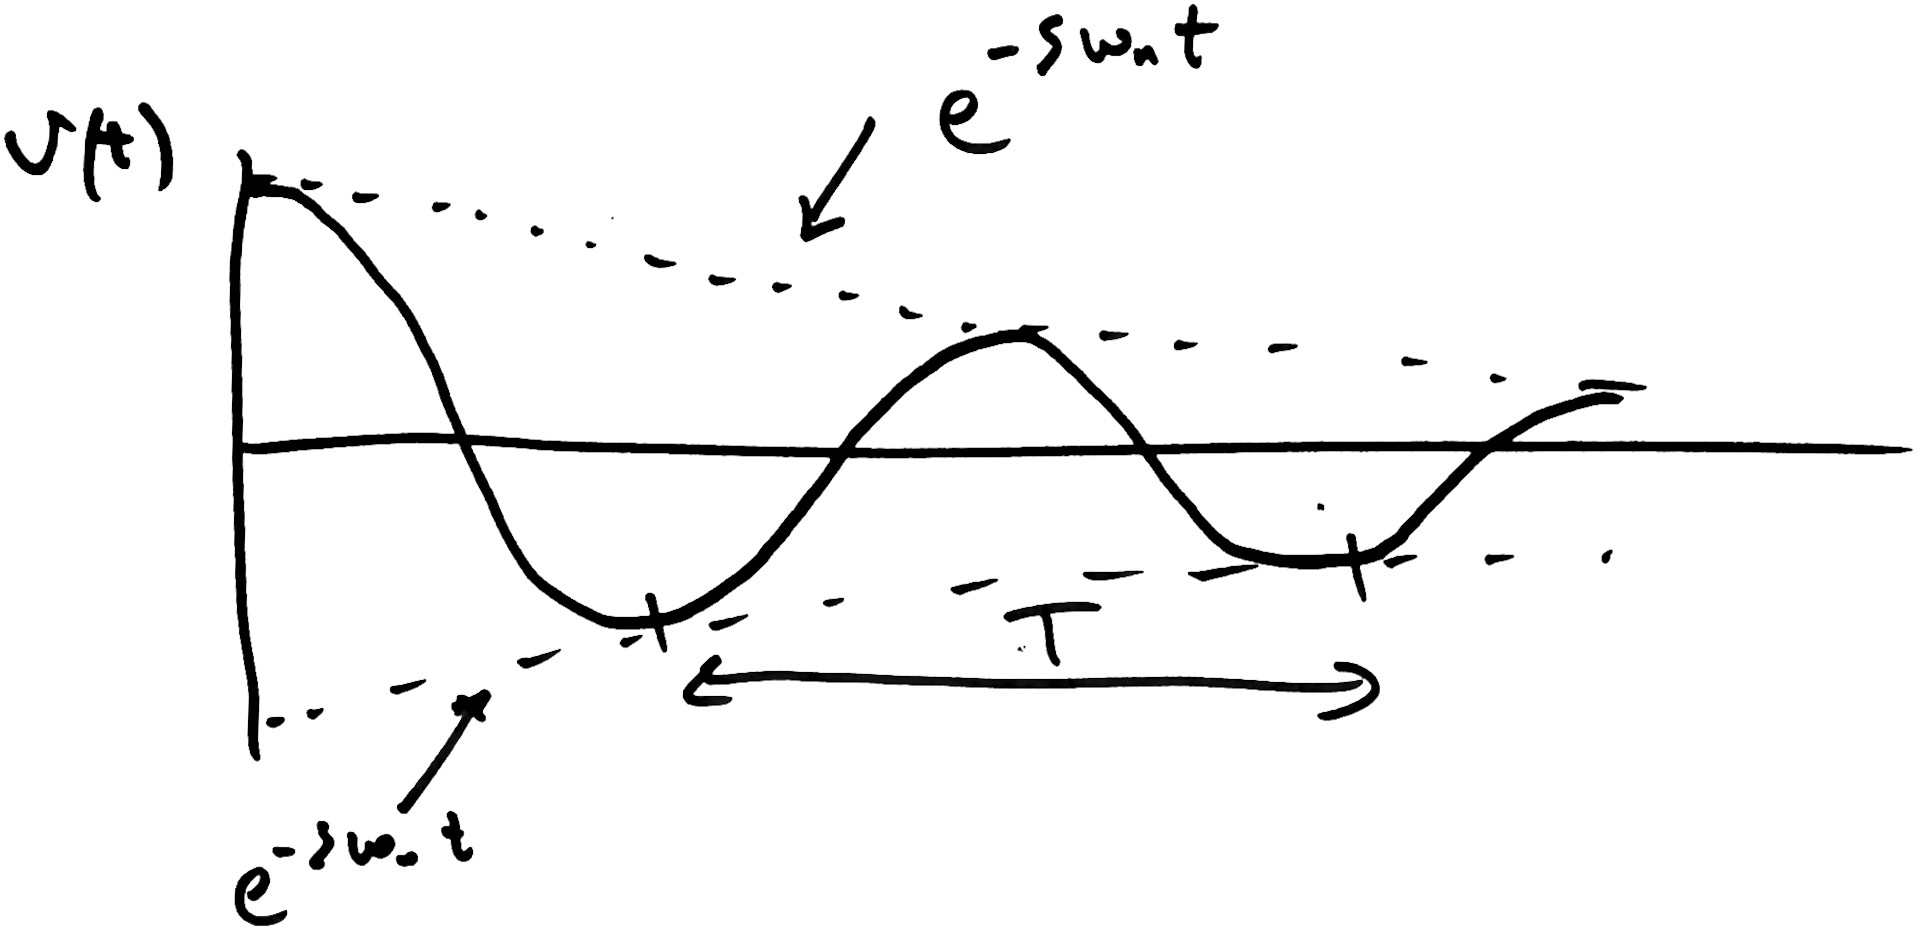
\includegraphics[width=0.7\linewidth]{figures/10/homo-resp}
  \caption{Homogeneous response of an LRC circuit with \(R > 0\).}
  \label{figure:lec10-homo-resp}
\end{figure}
With the same choices of \(\omega_n\) and \(\xi\), the eigenvalues of \(A\) can be expresssed as
\begin{align}
  \lambda_{1,2} &= -\xi \omega_n \pm j\omega_n \sqrt{1 - \xi^2}.
  % Initial conditions don't work so I just said "idk what the phase is"
  \intertext{The general form of the homogeneous response (modulo possible scaling and phase shift) is}
  v(t) &= \Re\cbr{e^{\lambda_1 t}} \\
  &= e^{-\xi\omega_n t} \Re\cbr{e^{j\omega_n \sqrt{1 - \xi^2} t}} \\
  &= e^{-\xi\omega_n t} \cos\del{\omega_n \sqrt{1 - \xi^2} t}
\end{align}
The graph of \(v(t)\), sketched in \autoref{figure:lec10-homo-resp}, is a sinusoid with period \(\frac{2\pi}{\omega_n \sqrt{1 - \xi^2}}\), trapped inside an exponential decaying at rate \(\xi \omega_n\).

\section{Reparameterized transfer function}
\begin{figure}
  \centering
  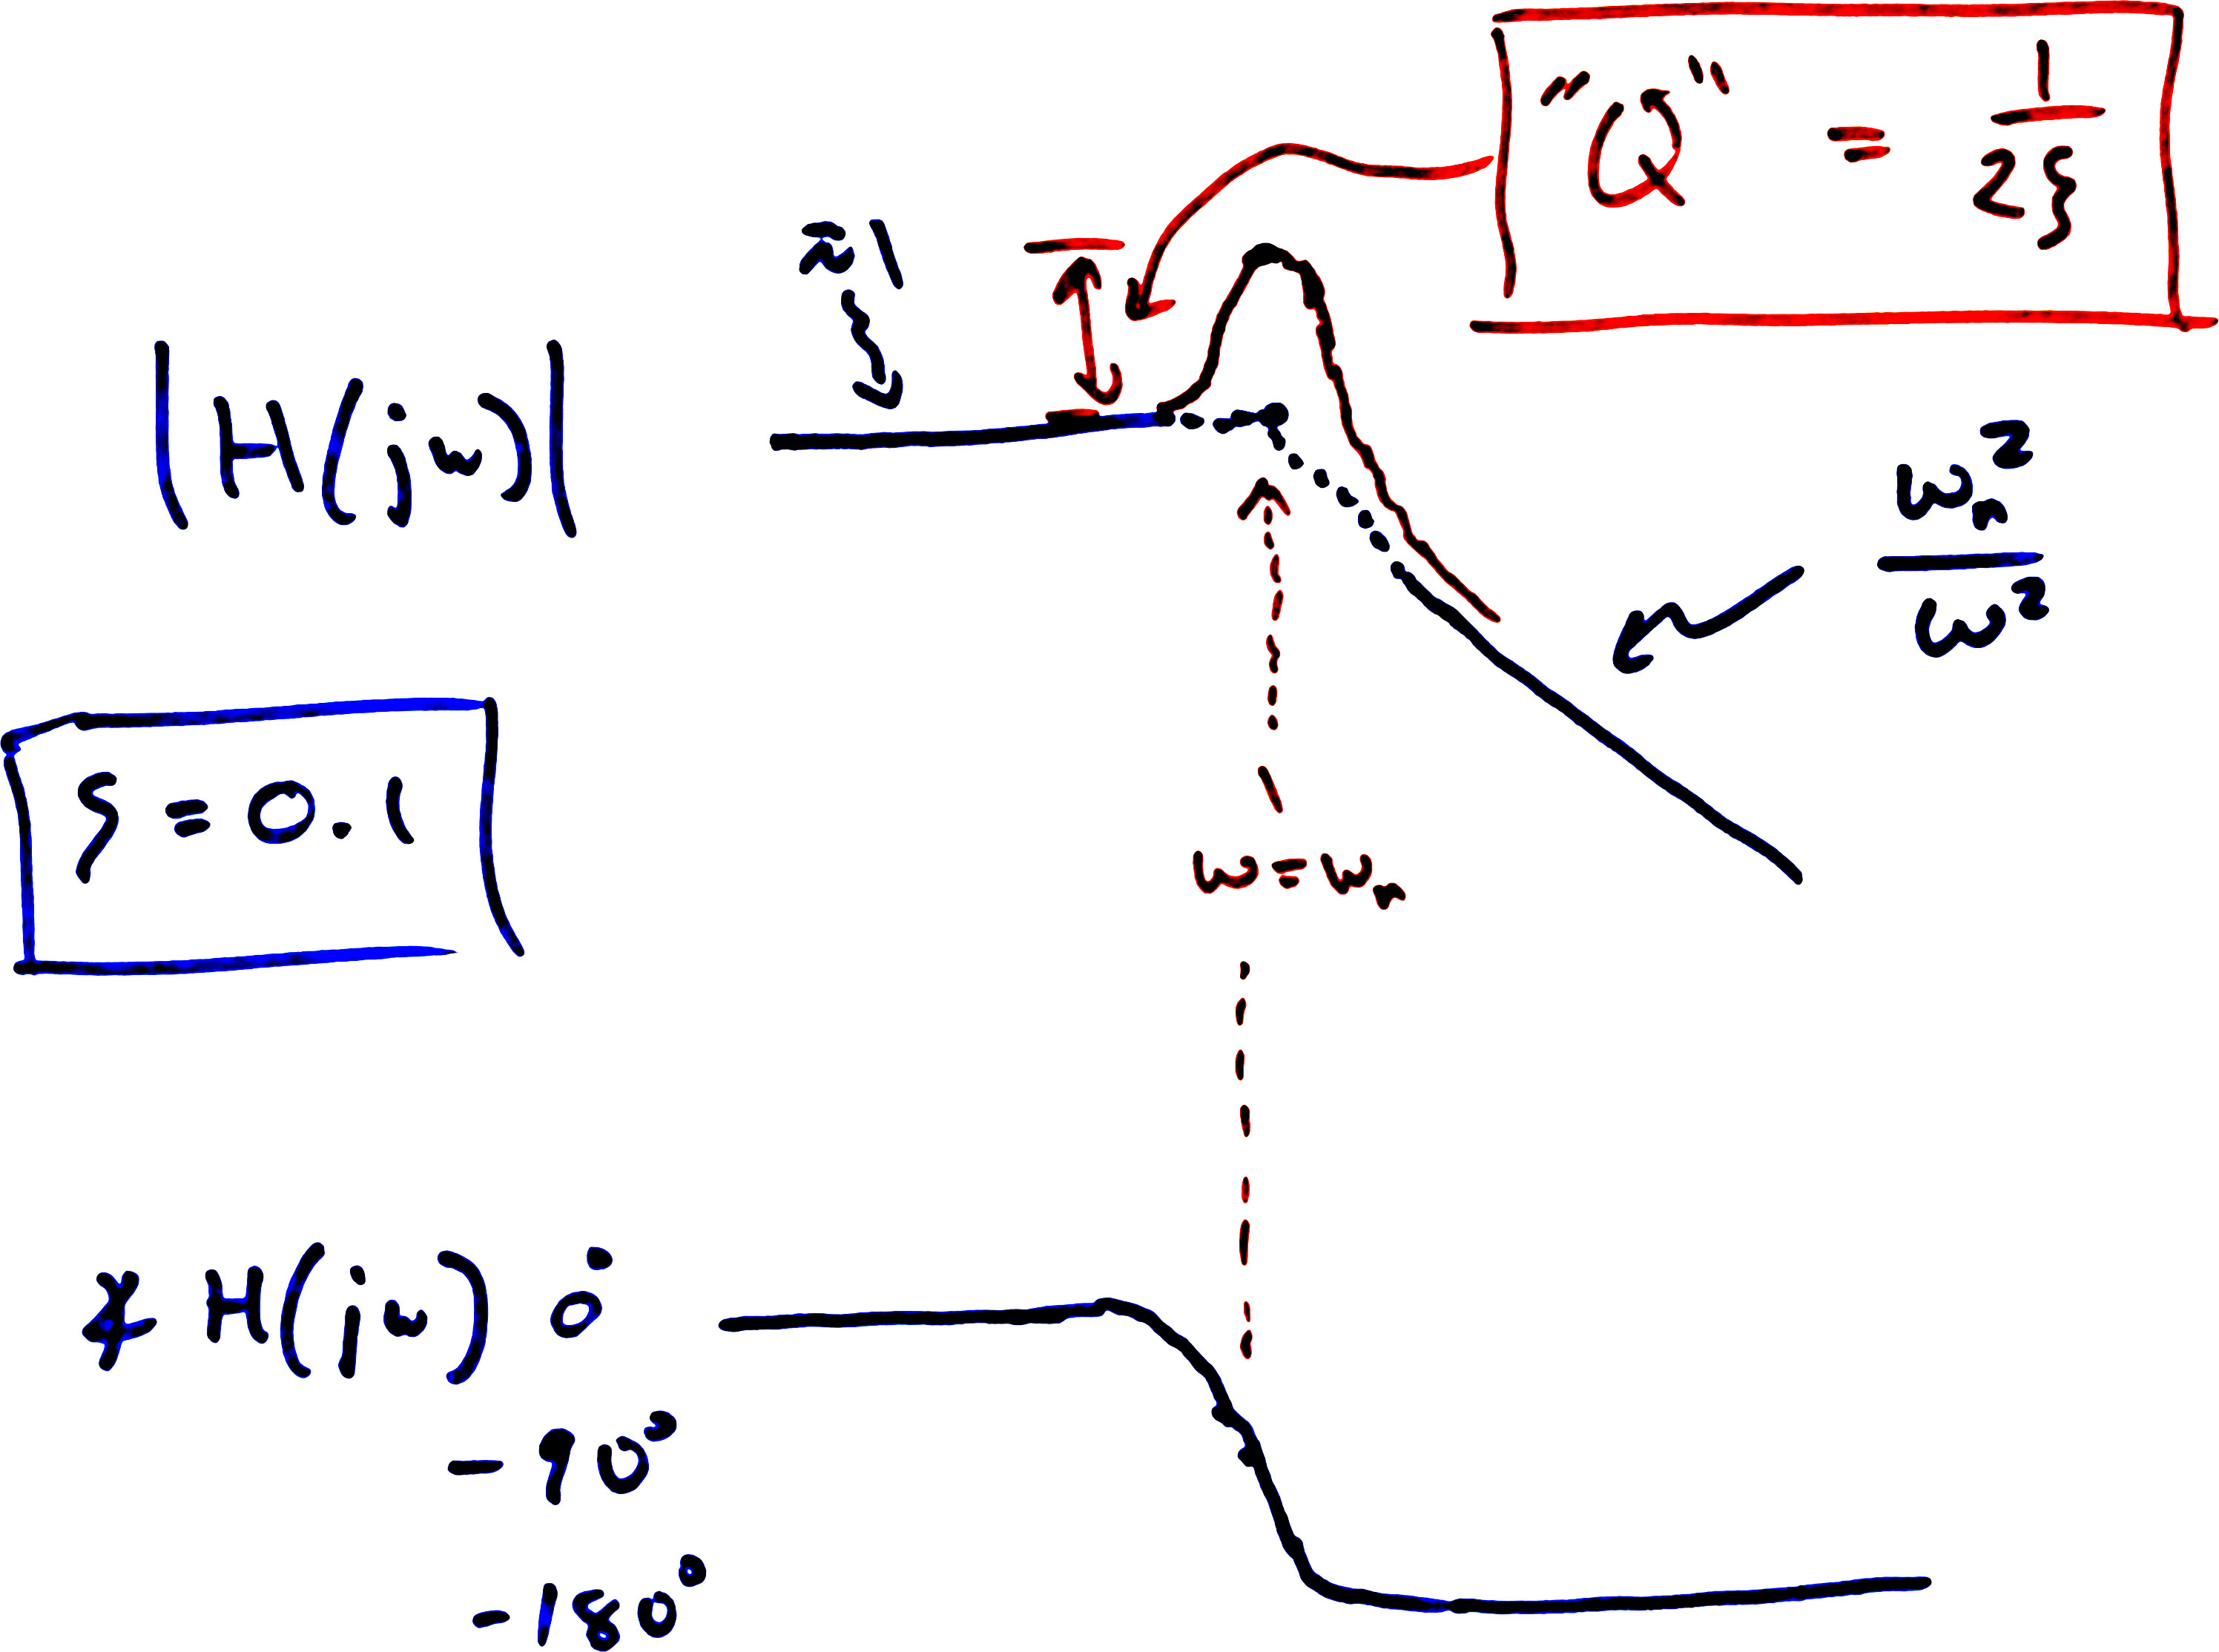
\includegraphics[width=0.8\linewidth]{figures/10/bode}
  \caption{Bode plot of an LRC filter with \(\xi = 0.1\).}
  \label{figure:lec10-bode}
\end{figure}
With the \(\omega_n\)-\(\xi\) parameterization, this circuit's transfer function becomes
\begin{align}
  \frac{V_\text{o}}{V_\text{in}}
  = H(j\omega)
  &= \frac{\omega_n^2}{\del{j\omega}^2 + \del{j\omega} 2 \xi \omega_n + \omega_n^2}
  \label{eq:lec10-LRC-tf}
\end{align}
We can imagine the Bode plot of \(H(j\omega)\) as having three pieces:
\begin{itemize}
  \item%[low frequencies]
  When \(\omega \ll \omega_n\), \(H(j\omega) \approx 1 \).
  \item%[resonant frequency]
  When \(\omega = \omega_n\), \(H(j\omega)  = \frac{-j}{2\xi}\). The magnitude is called ``Q.''%
  \footnote{Quality factor, or how selective this filter is of its favorite frequency.}
  \item%[high frequencies]
  When \(\omega \gg \omega_n\), \(H(j\omega)  \approx \frac{-\omega_n^2}{\omega^2}\).
\end{itemize}
A possible plot is shown in \autoref{figure:lec10-bode}.

\section{Applications of (R)LC filtering}
\subsection{Radio}
\begin{figure}
  \centering
  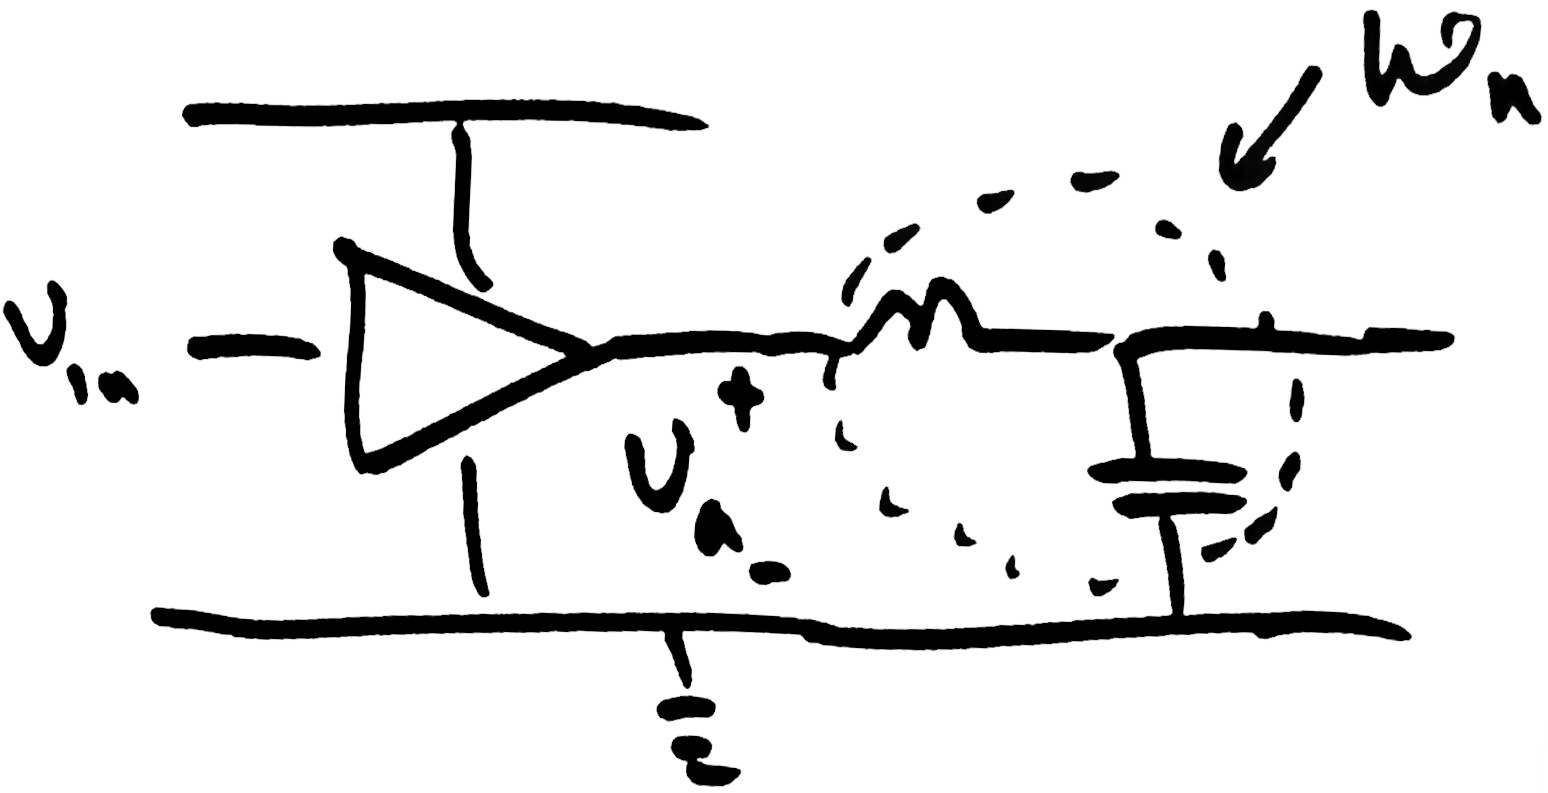
\includegraphics[width=0.6\linewidth]{figures/10/AM}
  \caption{An \(R\approx 0\) LC circuit used as an AM matching network.}
  \label{figure:lec10-AM}
\end{figure}

An AM radio antenna picks up a grab bag of electromagnetic signals, and to tune in to an AM radio channel, we need to detect the nonnegative function \(a(t)\) in front of its carrier wave \(\cos(\omega_n t)\).
A matching network as in \autoref{figure:lec10-AM} after the antenna improves the performance of a downstream amplifier around frequency \(\omega_n\) by altering the effective impedance of the antenna.%
\footnote{See \href{https://en.wikipedia.org/wiki/Impedance_matching}{impedance matching} on Wikipedia.}
\begin{align}
  v_\text{in} &= \underbrace{a(t)}_{\text{slow}} \ \underbrace{\cos(\omega_n t)}_\text{fast}
\end{align}
Taking the capacitor voltage as an output, we have \(\abs{v_\text{o}} \approx \frac{1}{2\xi} \abs{v_\text{a}}\).

\subsection{DC-DC converter}
\begin{figure}
  \centering
  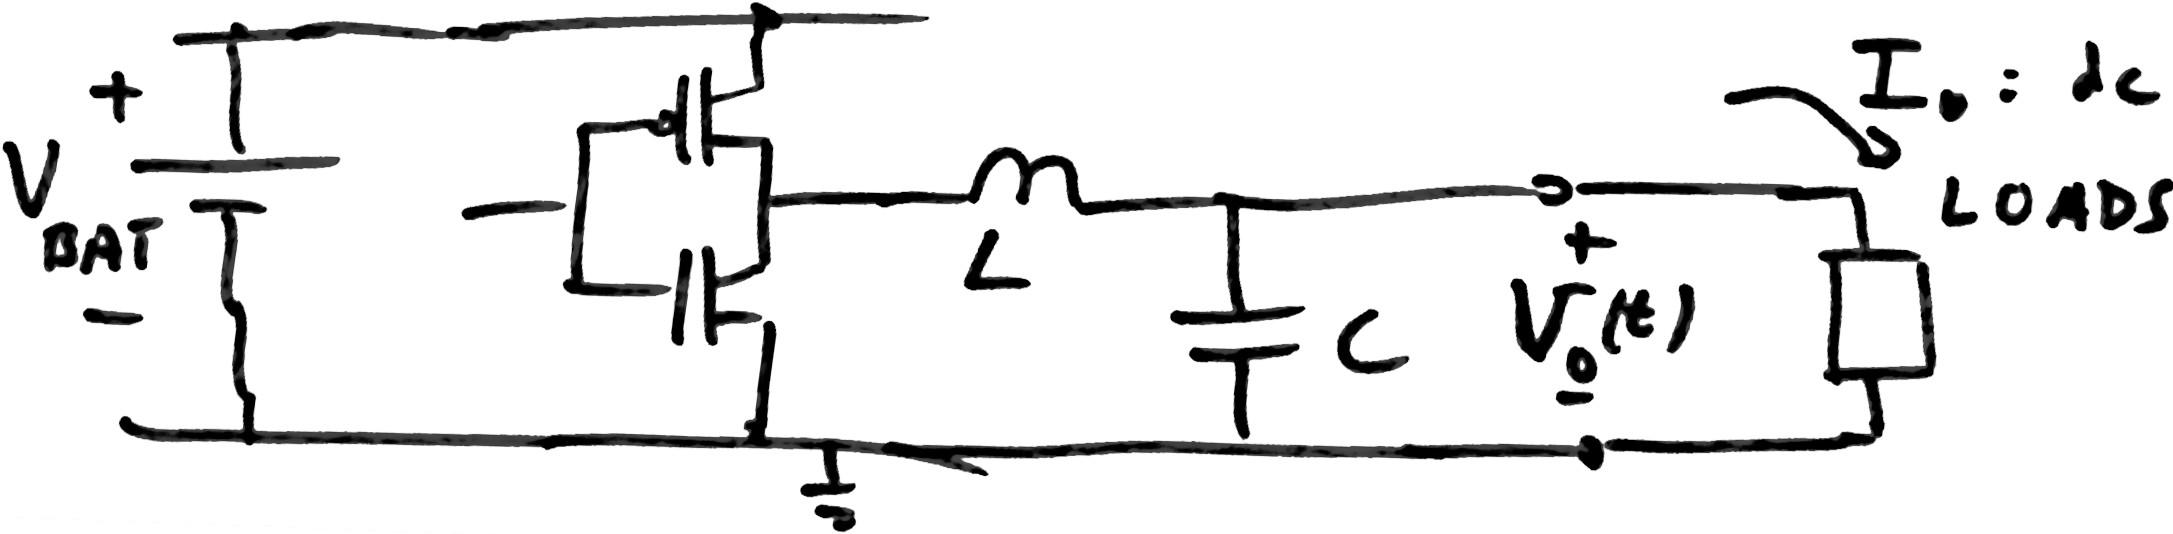
\includegraphics[width=1\linewidth]{figures/10/DC-DC}
  \caption{An \(R\approx 0\) LC circuit used in a DC-DC converter.}
  \label{figure:lec10-DC-DC}
\end{figure}
\begin{figure}
  \centering
  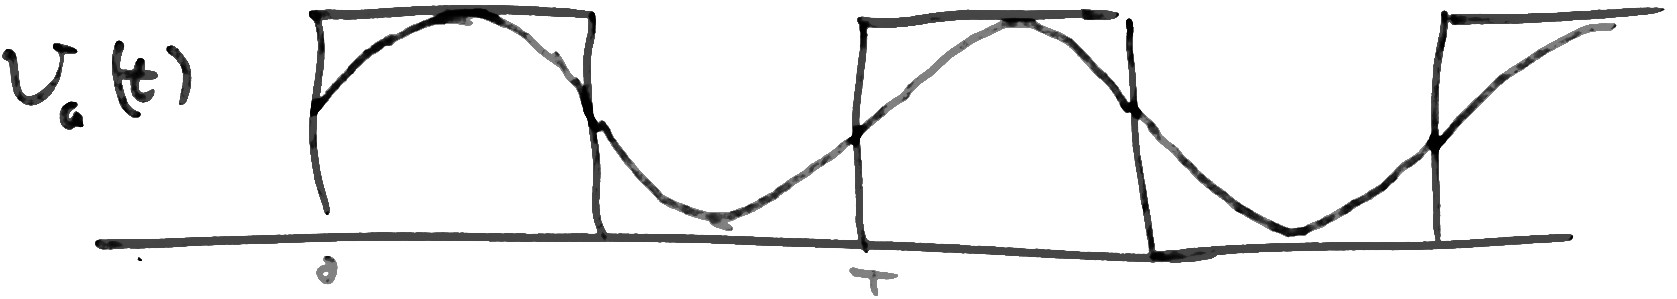
\includegraphics[width=1\linewidth]{figures/10/sqwave}
  \caption{Output of the switch in \autoref{figure:lec10-DC-DC}, approximated as an offset sine wave.}
  \label{figure:lec10-sq-approx}
\end{figure}
To step down a DC voltage source by 50\%, we can use a inverter operating
alternating at a 50\% duty cycle to generate an offset square wave whose DC component is the voltage we are trying to deliver.\footnote{For efficiency, we can use parallel NMOS and PMOS transistors on either side of the switch to reduce resistance. We also want an inductor with the smallest possible parasitic resistance.}
An LC filter reduces the AC component of the switch output, without dissipating power.

The inverter output \(v_\text{a}\) can be approximated as a sine wave with a DC offset (\autoref{figure:lec10-sq-approx}):
\begin{align}
  v_\text{a}(t)
  &= \underbrace{\frac{1}{2} V_\text{bat} \sin(\omega t)}_\text{ac} + \underbrace{\frac{1}{2} V_\text{bat}}_\text{dc}
  \intertext{We can use superposition to compute \(v_\text{o}\). The filter passes DC at unity gain, and it scales and shifts the AC component.}
  v_\text{o}(t)
  &= \frac{1}{2} V_\text{bat} + V_\text{o} \cos (\omega t + \phi)
\end{align}
In order to have a convincing DC output, we need \(V_\text{o} \ll V_\text{bat}\).
That sinusoid, as well as everything else that makes a square wave a square wave, will have to fit into the \(\abs{H(j\omega)} \approx \frac{\omega_n^2}{\omega^2}\) high-frequency region of \autoref{eq:lec10-LRC-tf}.
That means we need to choose an \(\omega_n\) such that \(\omega_n \ll \omega\).
For the DC amplitude to exceed the AC ``ripple'' amplitude by a factor of 100, for instance, \(\omega\) would have to exceed \(10\omega_n\).
